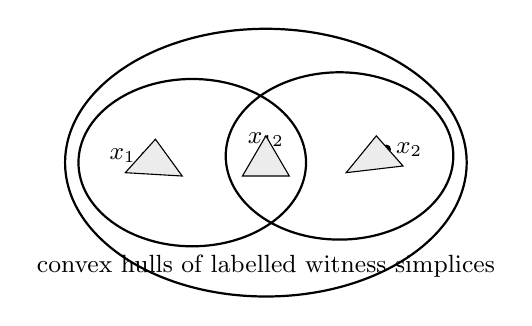
\begin{tikzpicture}[scale=.85,font=\small]
\draw[thick] (0,0) ellipse (3 and 2);
\draw[thick] (-1.1,0) ellipse (1.7 and 1.25);
\draw[thick] (1.1,.1) ellipse (1.7 and 1.25);
\fill (-1.8,.1) circle (2pt) node[left]{$x_1$};
\fill (1.8,.2) circle (2pt) node[right]{$x_2$};
\fill (0,.1) circle (2pt) node[above]{$x_{12}$};
\draw[fill=gray!15] (-2.1,-.15)--(-1.65,.35)--(-1.25,-.2)--cycle;
\draw[fill=gray!15] (1.2,-.15)--(1.65,.4)--(2.05,-.05)--cycle;
\draw[fill=gray!15] (-.35,-.2)--(0,.4)--(.35,-.2)--cycle;
\node at (0,-1.55) {convex hulls of labelled witness simplices};
\end{tikzpicture}